\documentclass[12pt,a4paper]{article}
\usepackage[utf8]{inputenc}
\usepackage[francais]{babel}
\usepackage[T1]{fontenc}
\usepackage{amsmath}
\usepackage{amsfonts}
\usepackage{amssymb}
\usepackage{float}
\usepackage{graphicx}
\author{Baptiste Lesquoy}
\begin{document}
\part{Élaboration du protocole}
\section{Objectif}
On aimerait définir un protocole qui permettrait de mesurer précisément un décalage de phase sur un signal enregistré en même temps par deux micros différents.


\section{Expérience}
\subsection{Critères d'acceptation}
On considérera que le protocole est bon si on arrive systématiquement et dans plusieurs configurations à retrouver les distances physiques séparant l'émetteur du signal de chacun des micros. De plus on vérifiera que le décalage de phase entre les micros correspond bien à la distance les séparant.

\subsection{Configurations}
Tout au long du document, on utilisera les termes m1 et m2 pour désigner les deux micros, x l'espace entre les micros, s1 la source sonore (le haut parleur), et y la distance entre m2 et s1. De sorte que la configuration avec les micros et le haut parleur aligné puisse être schématisé comme si dessous:
\begin{figure}[H]
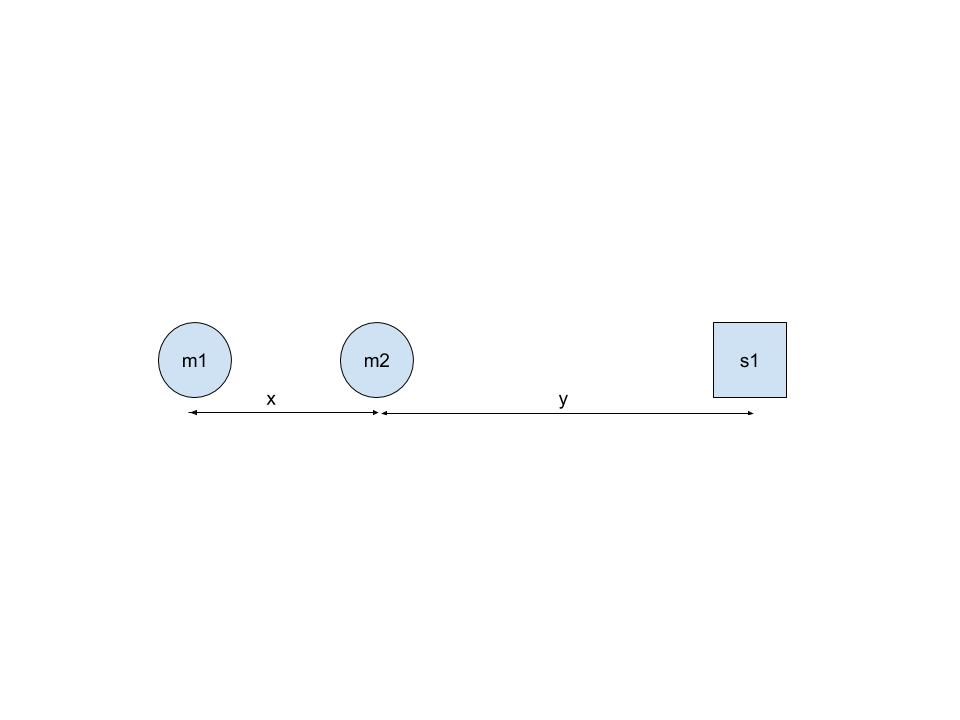
\includegraphics[width=\textwidth]{../24-02-16/mesures/m1/schema.png} 
\caption{Schéma de l'expérience avec les micros et le haut parleur alignés}
\end{figure}
les différentes configurations choisies sont:
\begin{itemize}
\item m1, m2 et s1 sont alignés, on teste différentes valeurs de x et y.
\item m1 et m2 sont côte à côte, plus ou moins collés.
\end{itemize}
\subsection{Signal émit}
On utilisera un fichier sonore wav qui:
\begin{itemize}
\item dure 3 secondes
\item est un sinus à une fréquence constante a 300Hz
\item a un sample rate de 44100Hz
\item est un fichier mono
\end{itemize}
Le signal est émit depuis une enceinte branché à un ordinateur via une prise jack 3.5.



\subsection{Réception du signal}
Le signal est enregistré via deux micros identiques (même modèle), posés sur de la mousse. Le tout est coordonné par un contrôleur trik sur lequel les micros sont branchés via deux prises jack 3.5 séparées.
On enregistre le signal réceptionné dans un fichier wav avec un taux d'échantillonnage de 192000Hz.
Chaque enregistrement dur 6 secondes, on commence par démarrer l'enregistrement, puis on attend une à 2 secondes avant d'émettre le signal. Ainsi on peut observer le bruit ambiant et être sûr de capter l'intégralité du signal émit.
Les calculs de distances et de décalage de phase seront fait par rapport aux premiers samples reçu du signal, afin de ne pas être influencé par l'écho.

\section{Résultats/conclusions}
\subsection{Tout aligné}
\begin{figure}[H]
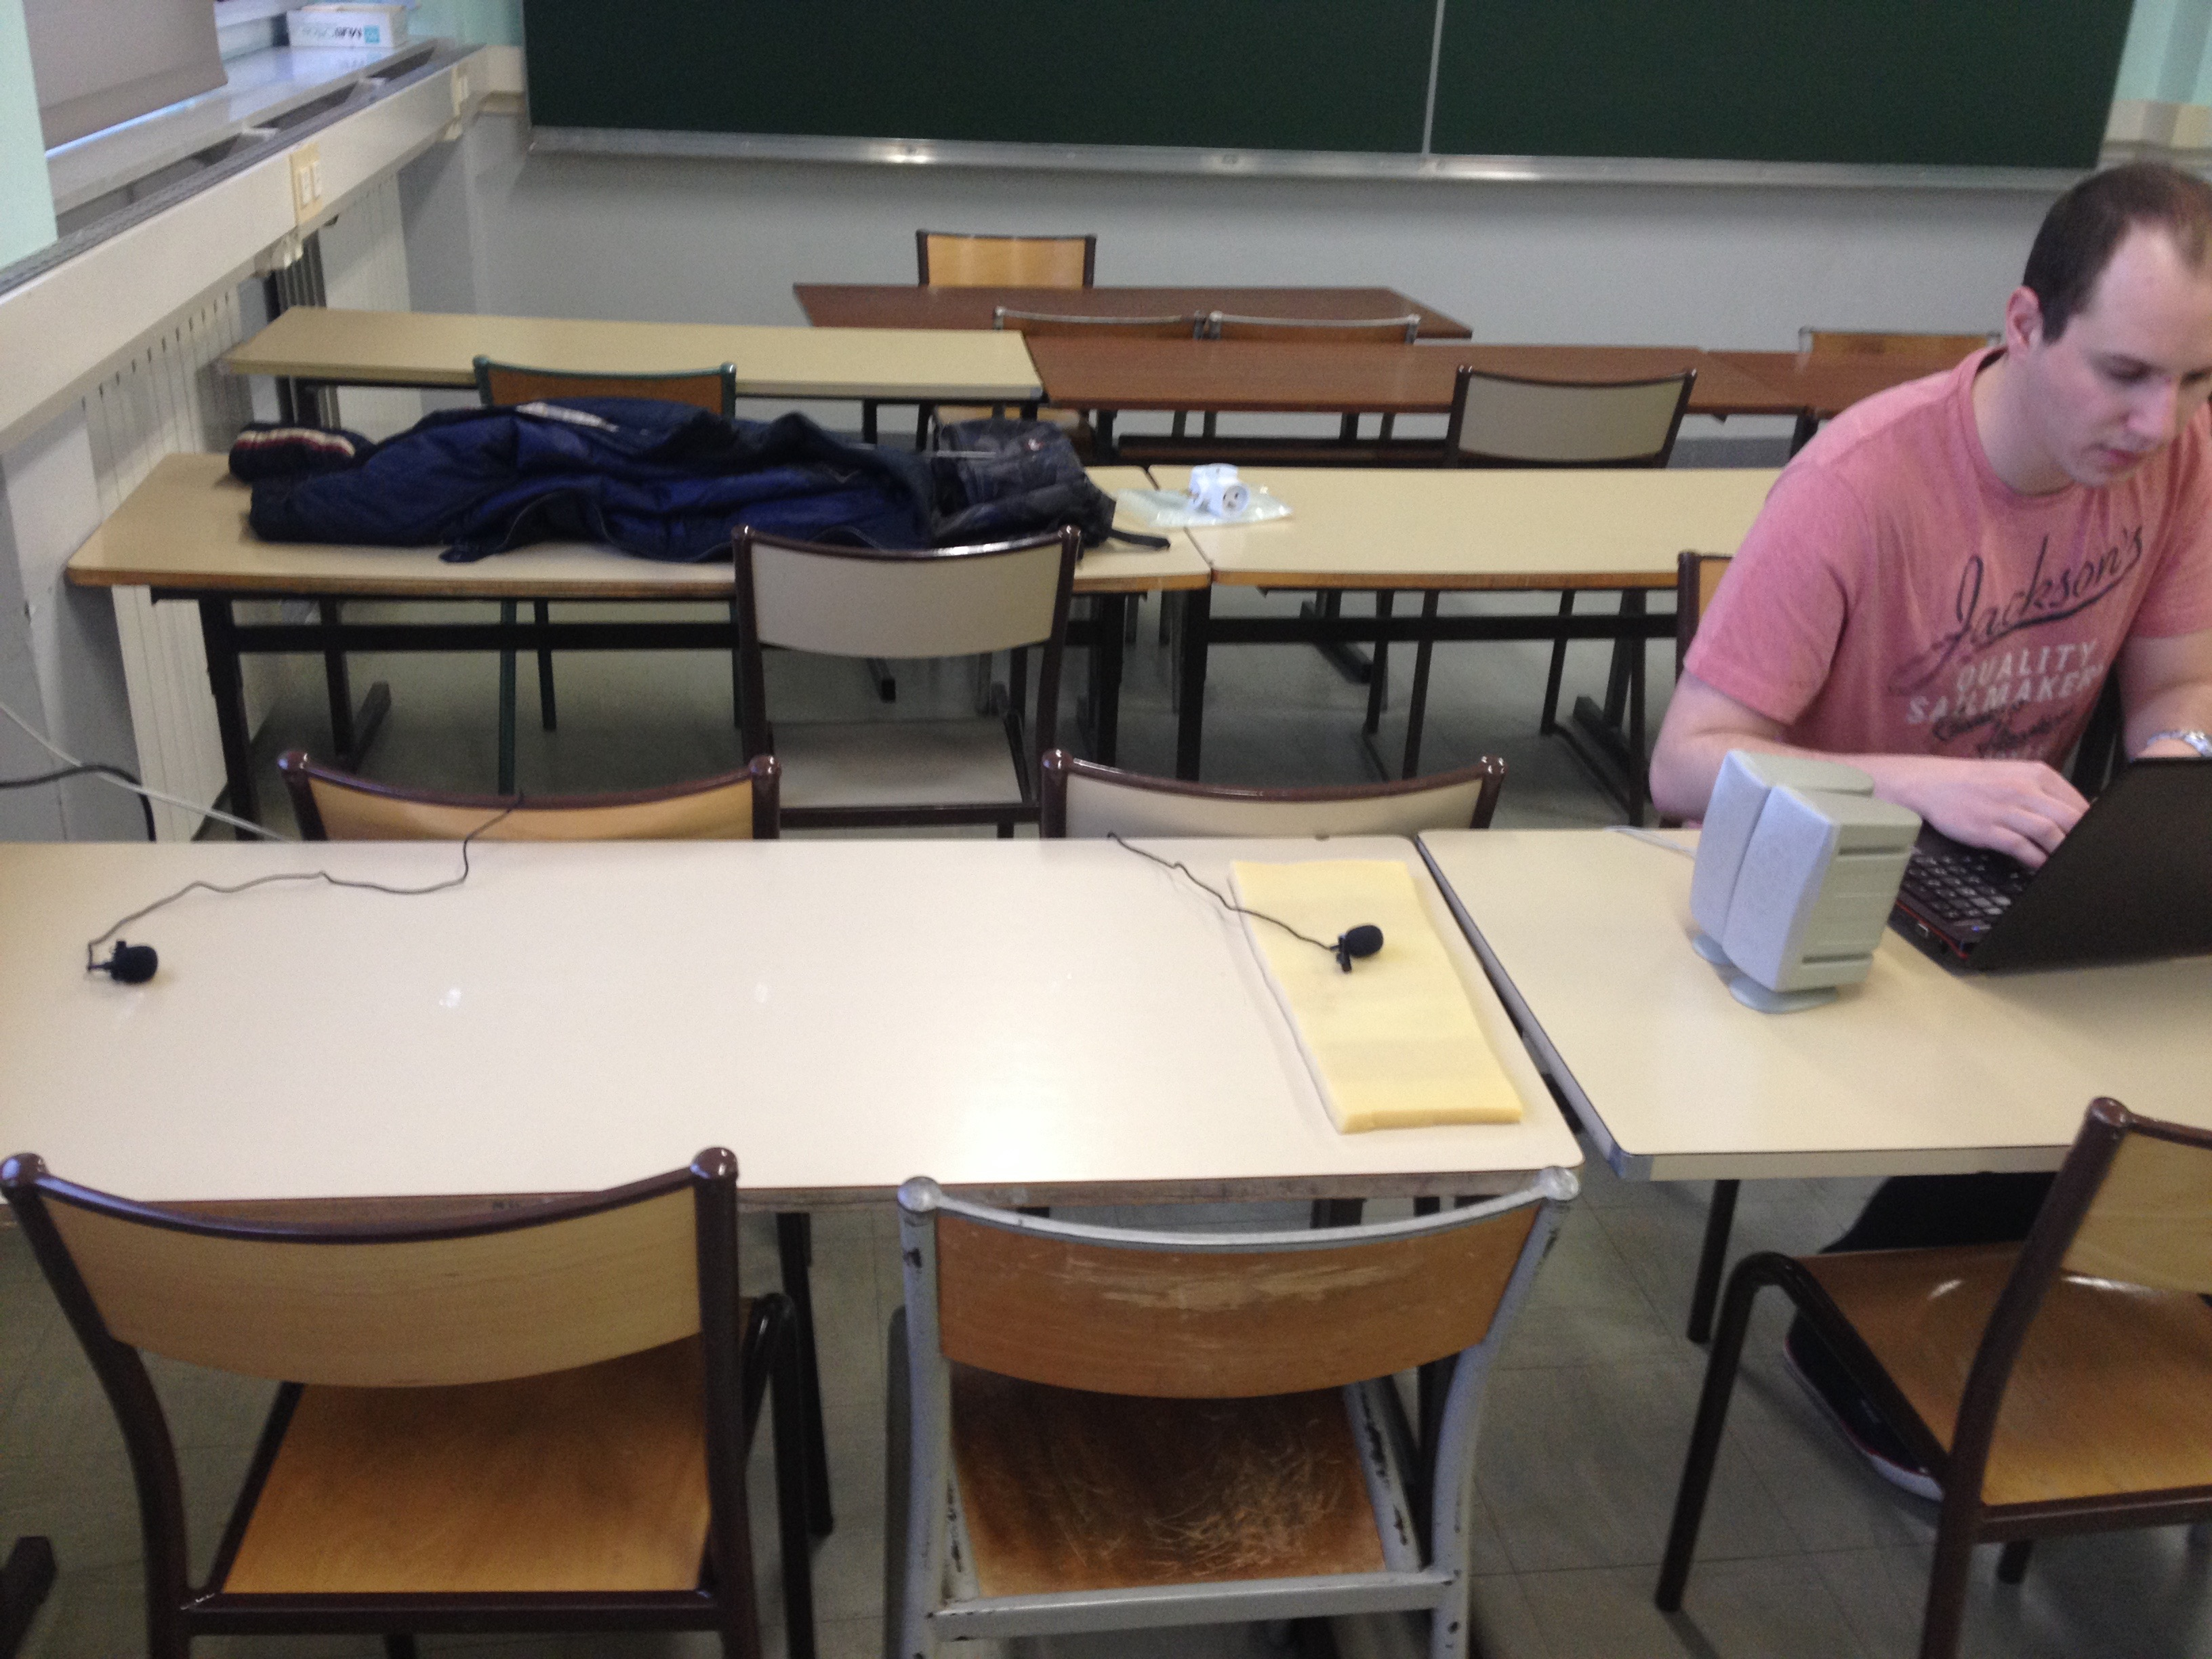
\includegraphics[width=\textwidth]{../donnees25-02/IMG_0919.jpg} 
\caption{expérience avec les micros et l'enceinte aligné}
\end{figure}
\begin{figure}[H]
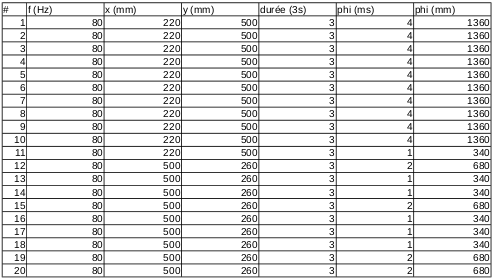
\includegraphics[width=\textwidth]{../donnees25-02/mesures_en_ligne/tableau_resultats.png}
\caption{tableau des résultats de toutes les itération de l'expérience avec les micros et enceintes alignés}
\end{figure}
On constate que le décalage de phase correspond aux distances entre m1, m2 et s1\\
TODO: exprimer le décalage en sample pour des distances plus précises + ce serait sympa de retrouver la formule, parce que phi ça ne me parle pas trop sans contexte :)

\subsection{Récepteurs côte à côte}
\begin{figure}[H]
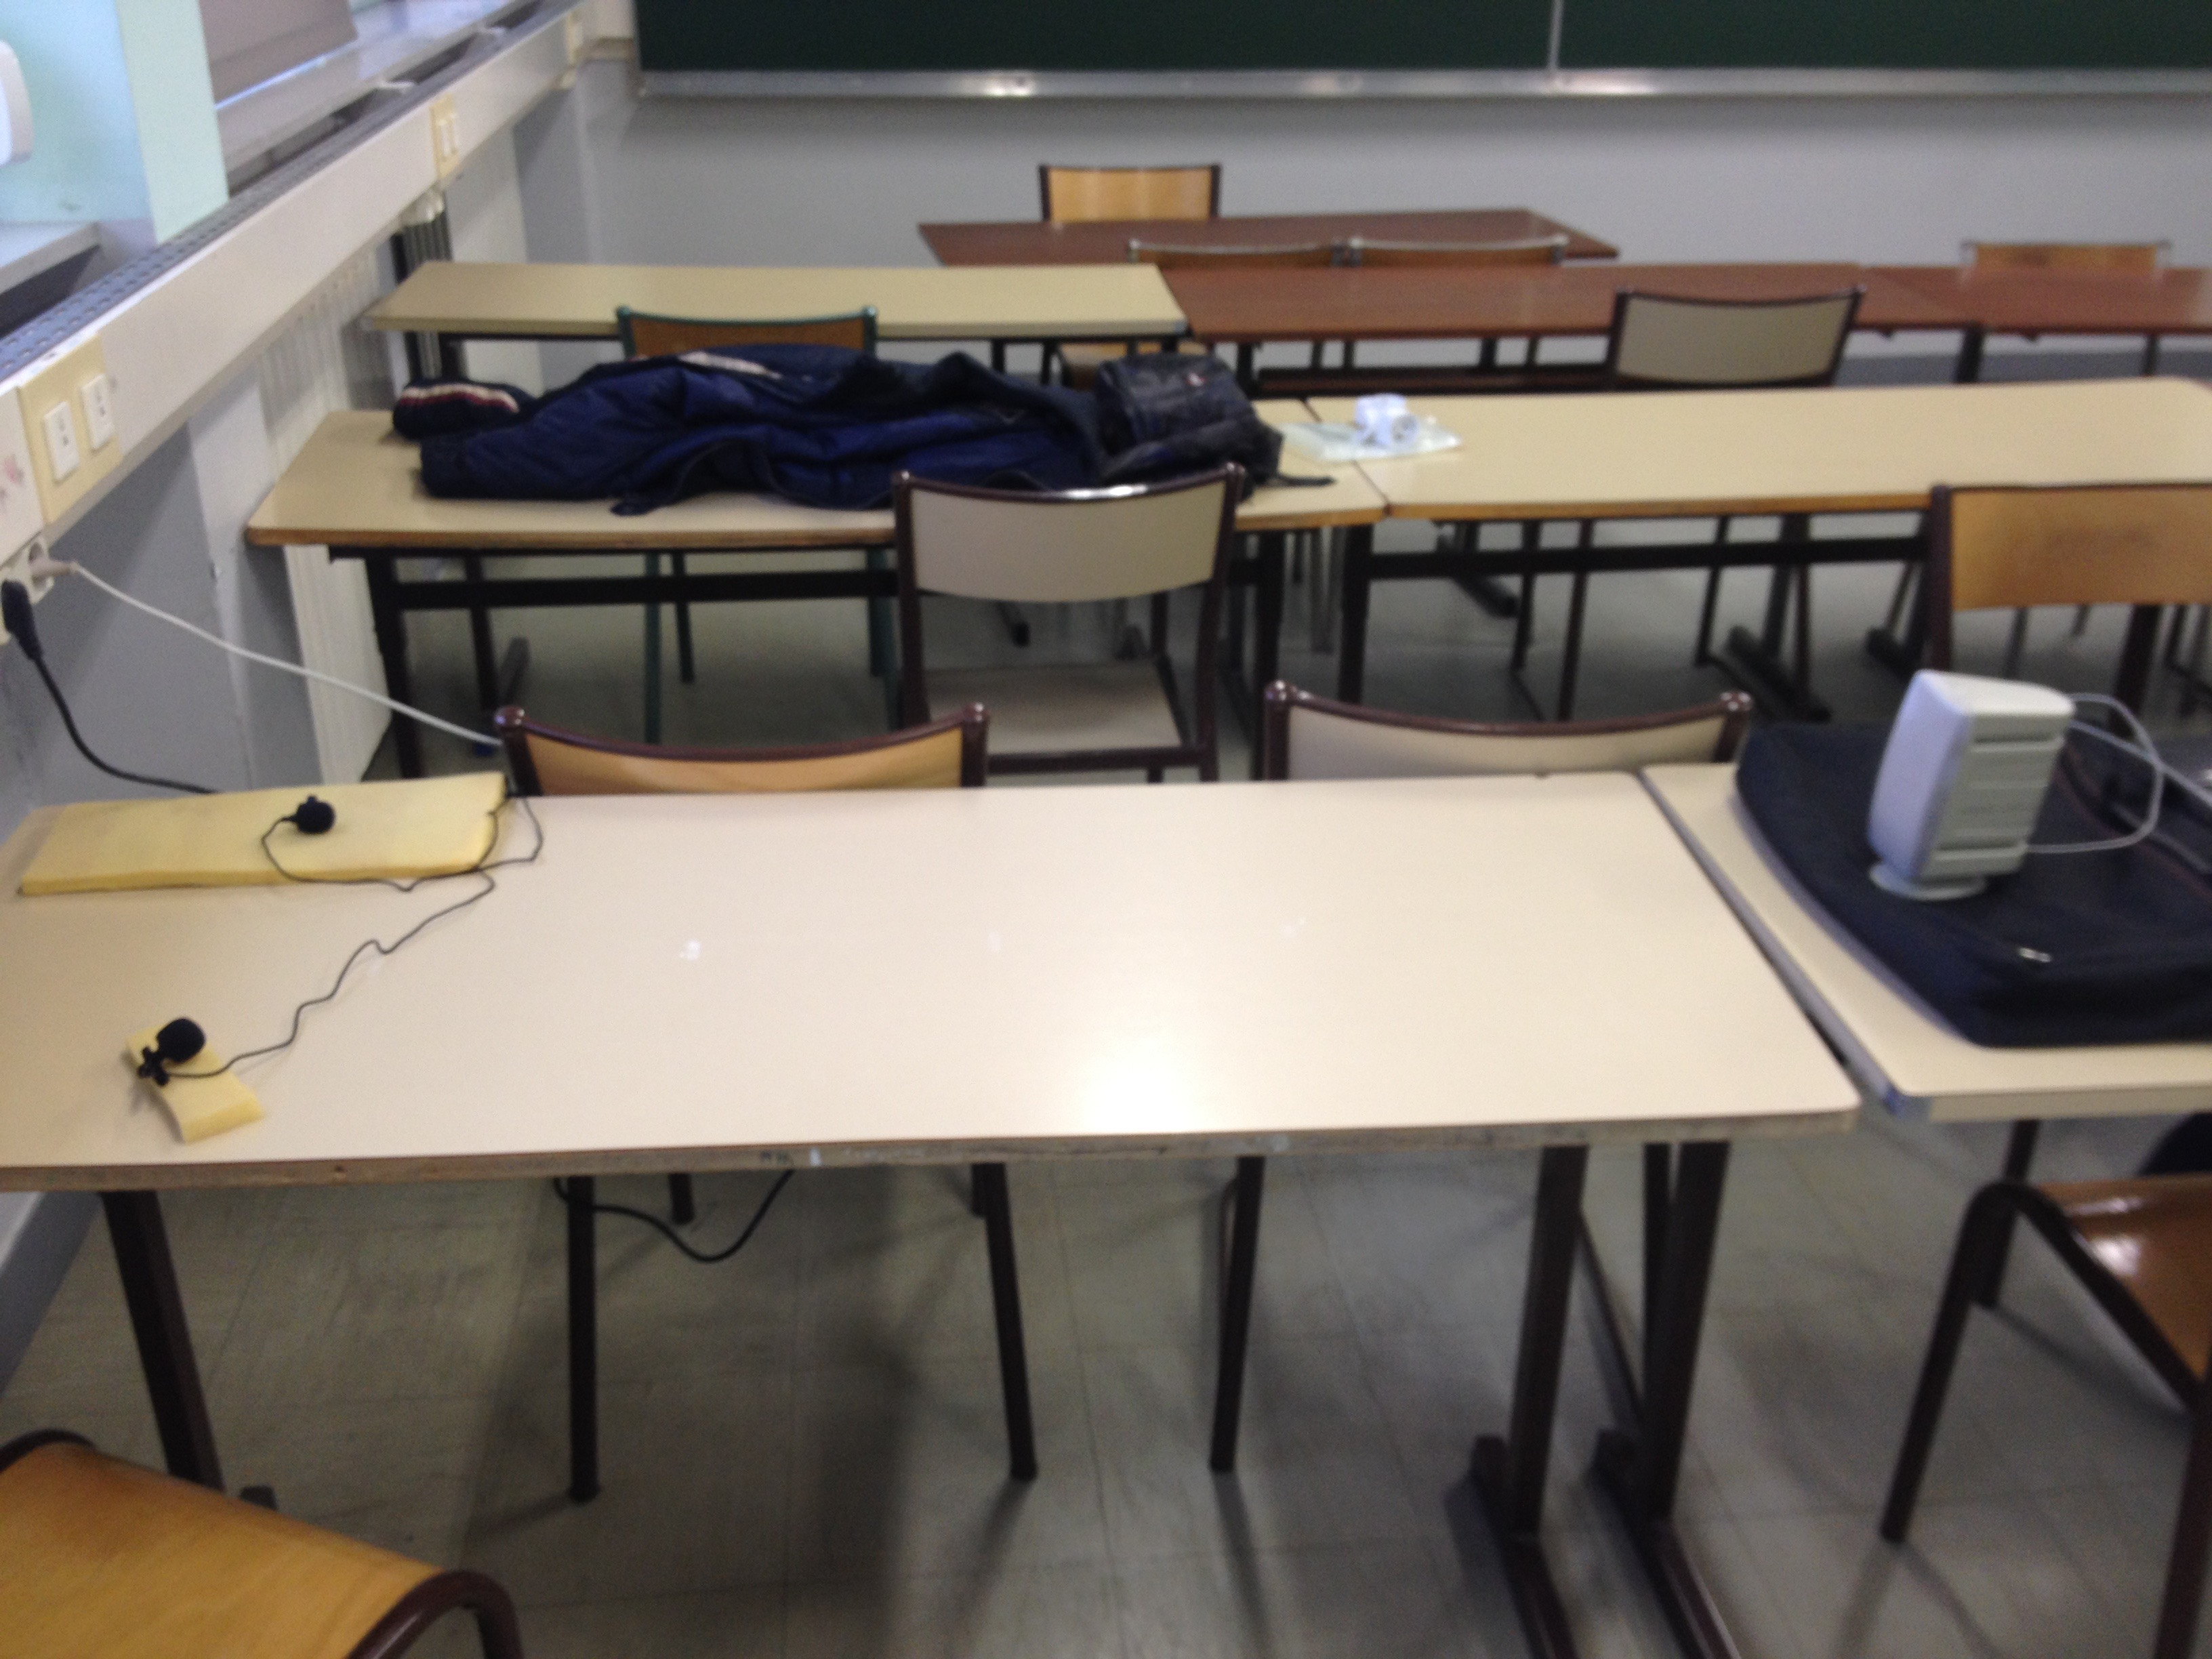
\includegraphics[width=\textwidth]{../donnees25-02/IMG_0920.jpg} 
\end{figure}

\begin{figure}[H]
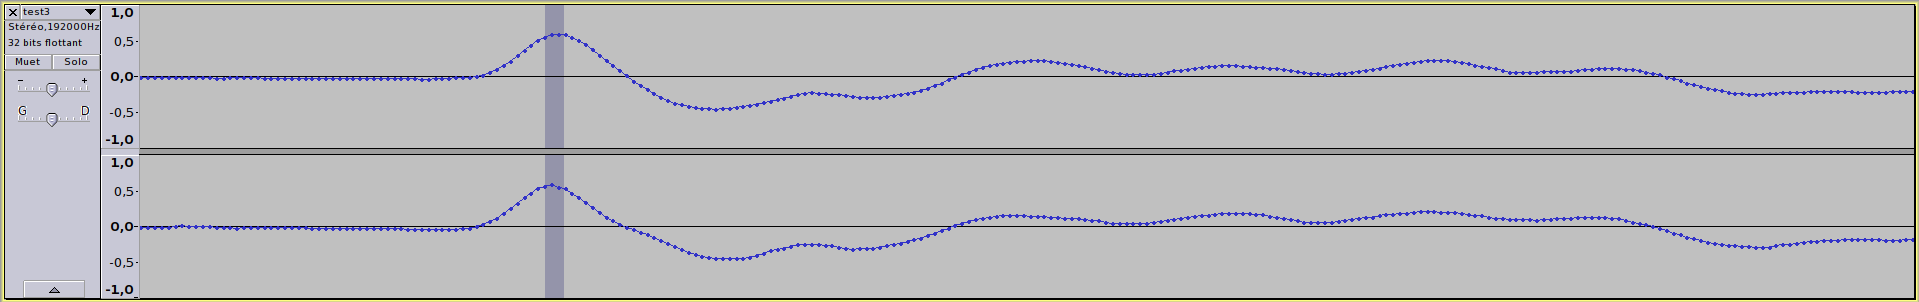
\includegraphics[width=\textwidth]{../donnees25-02/mesures_micro_colles/colles.png} 
\caption{signaux reçu par les deux micros lorsqu'ils sont collés}
\end{figure}
On constate bien qu'il n'y a pas de décalage quand les deux micros sont collés. Par contre on remarque une différence d'intensité, qui peut être expliqué par une simple différence du matériel. Les micros n'étant pas des micros professionnels, ce n'est pas étonnant que la qualité ne soit pas constante d'un micro à l'autre.


TODO: même chose que précédemment :)


\part{Décalage de phase}
\section{Objectif}
Dans l'expérience précédente on a ignoré l'écho, cette fois si, on aimerait savoir à quel point l'écho peut avoir de l'importance dans le signal reçu, et plus particulièrement dans le décalage de phase entre les deux micro .
On va donc utiliser de la mousse pour rendre les micros plus "directionnels" et regarder si ça a de l'influence sur les données enregistrées selon la direction donné.

\section{Expérience}
\subsection{Critères d'acceptation}
On commencera par reprendre la dernière configuration de l'expérience précédente en ajoutant un cône autour d'un des micros afin de vérifier que le signal reçu est différent avec et sans le cône (donc que la mousse est bien efficace pour filtrer le signal).
On considérera que l'écho a de l'influence sur le signal reçu si en changeant l'orientation d'un micro placé dans un cône en mousse on observe un décalage de phase différent par rapport à un micro sans cône (donc omnidirectionnel).

\subsection{Configurations}
On reprend la configuration précédente. Cette fois, on placera les micros côte à côte et on changera uniquement l'orientation  du micro entouré d'un cône de mousse.

\subsection{Signal émit et réception}
Le matériel et les paramètres sont les mêmes que pour l'expérience précédente à la seule différence du cône en mousse autour d'un des micros.

\section{Résultats/conclusions}


\subsection{Vérification de l'efficacité de la mousse}
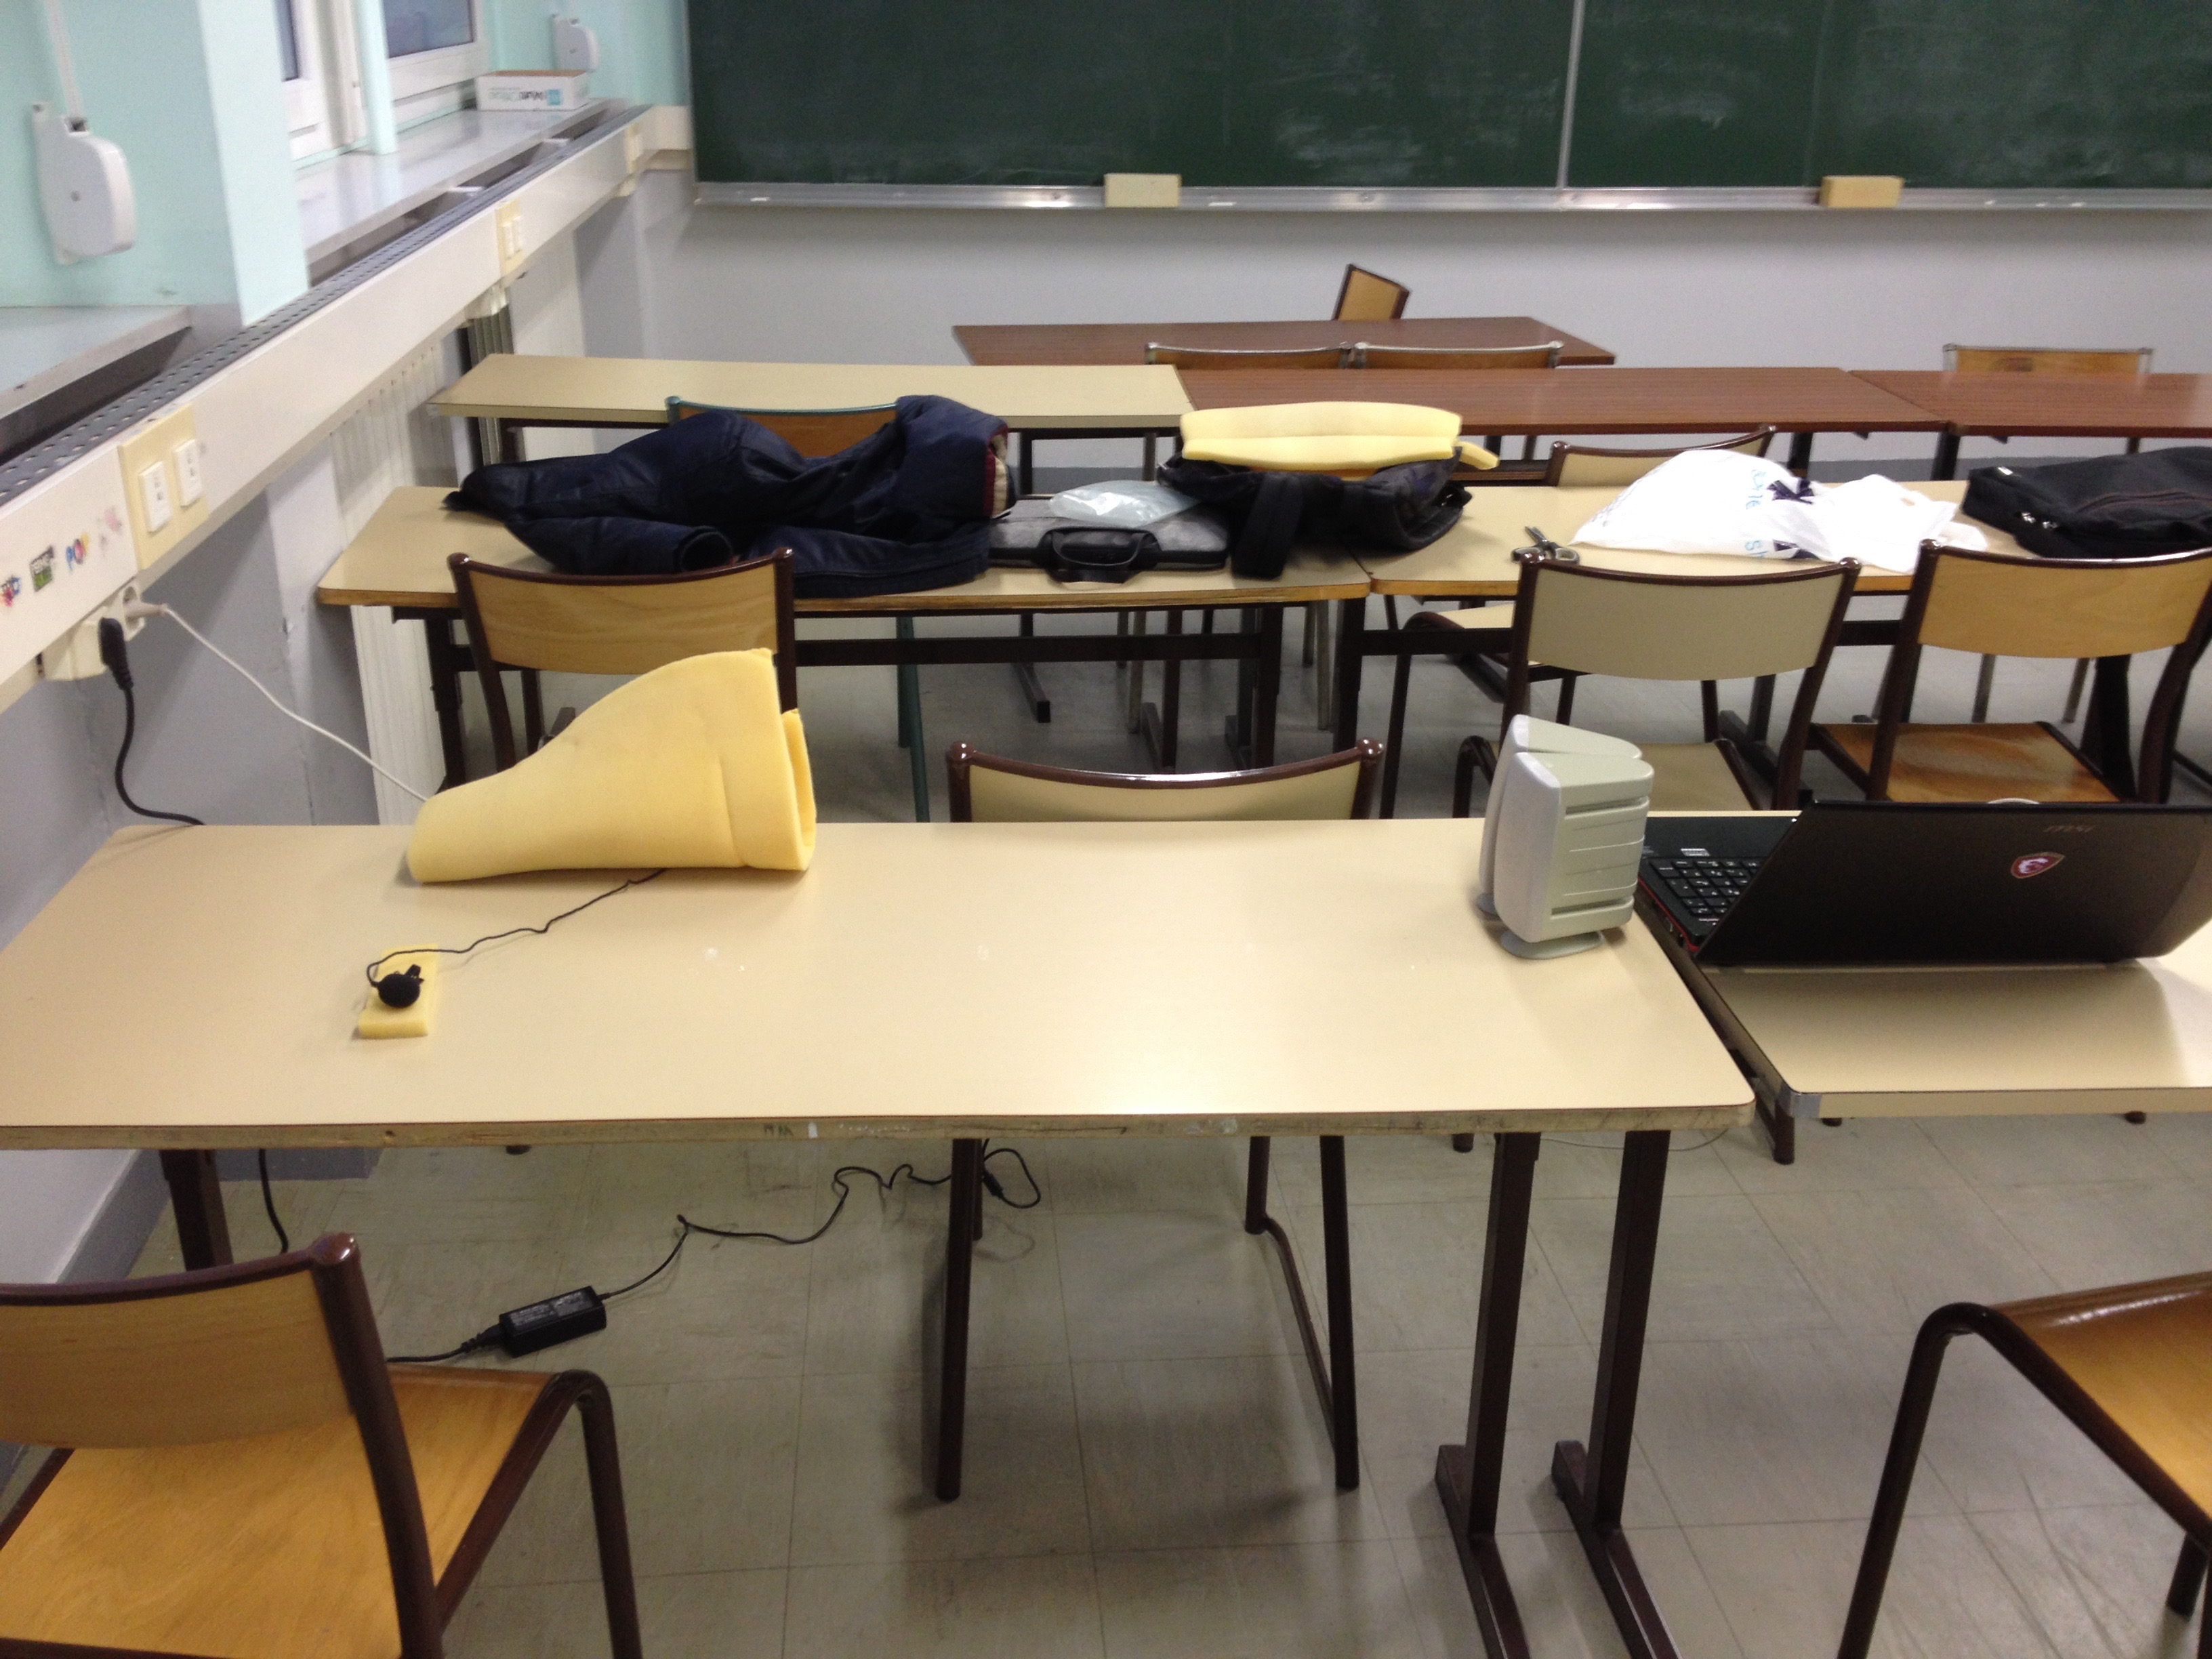
\includegraphics[width=\textwidth]{../donnees25-02/IMG_0922.jpg} 

\subsection{Changement d'orientation}


\begin{figure}[H]
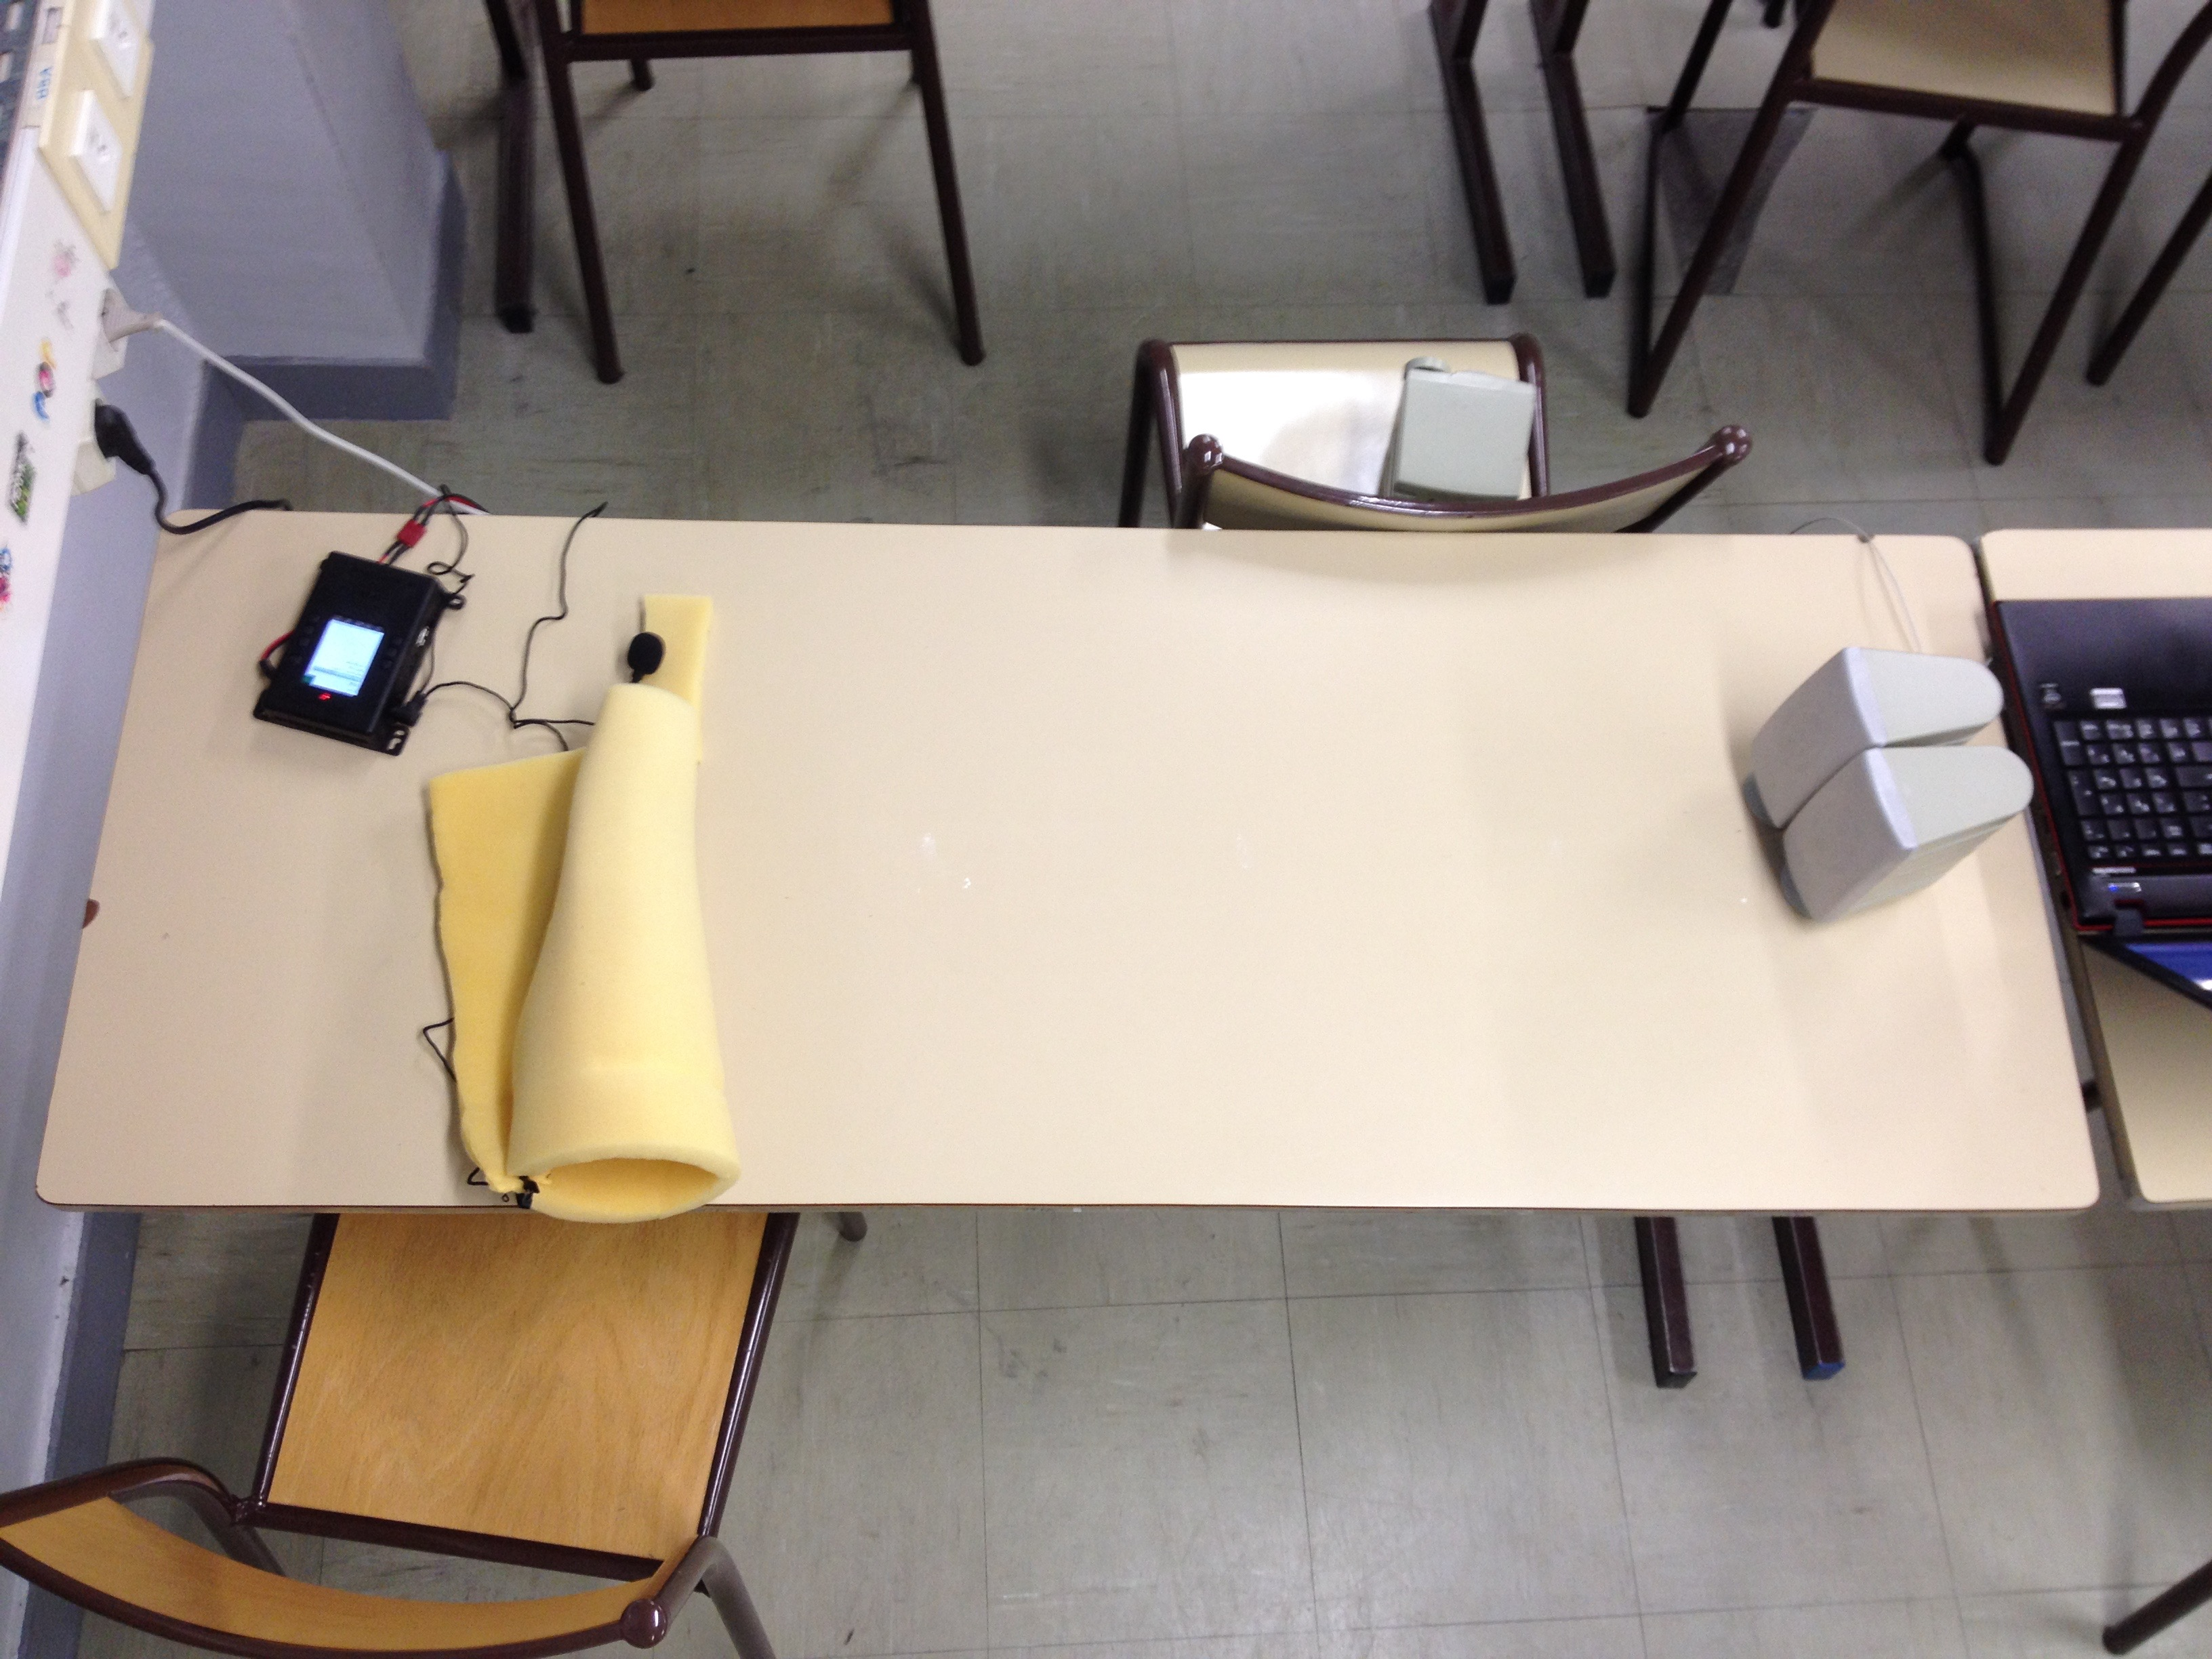
\includegraphics[width=\textwidth]{../donnees25-02/IMG_0923.jpg} 
\end{figure}


\paragraph{perpendiculaire au haut parleur}

On constate déjà qu'il y a un décalage assez marqué(anormal puisque les micros sont côte à côte)
\begin{figure}[h]
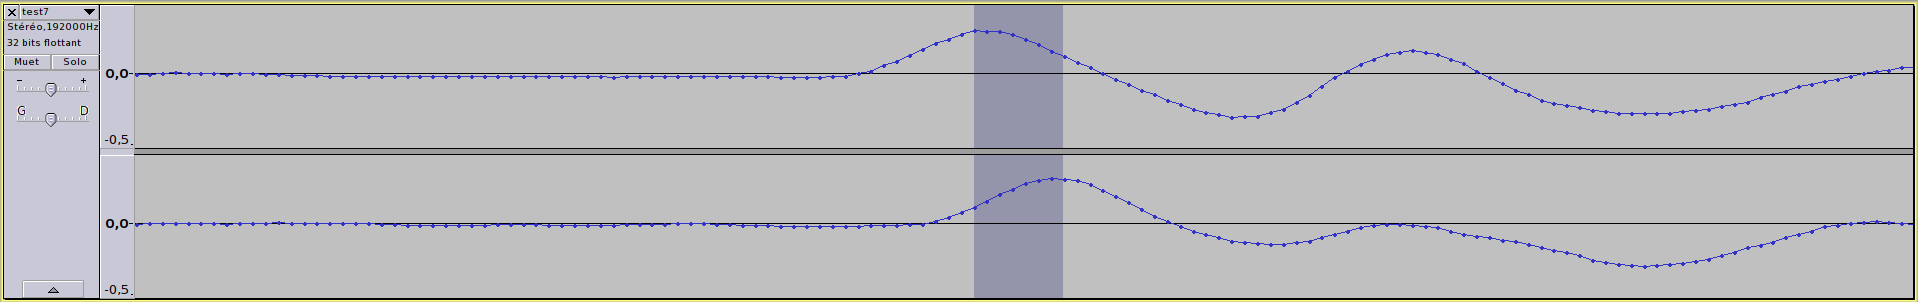
\includegraphics[width=\textwidth]{../donnees25-02/mesures_perpendiculaires/test7.png} 
\caption{exemple de décalage sur la 7ème itération de l'expérience}
\end{figure}

TODO: faire le tableau avec tous les décalages, calculer le décalage moyen

\paragraph{dos au haut parleur}

\begin{figure}[H]
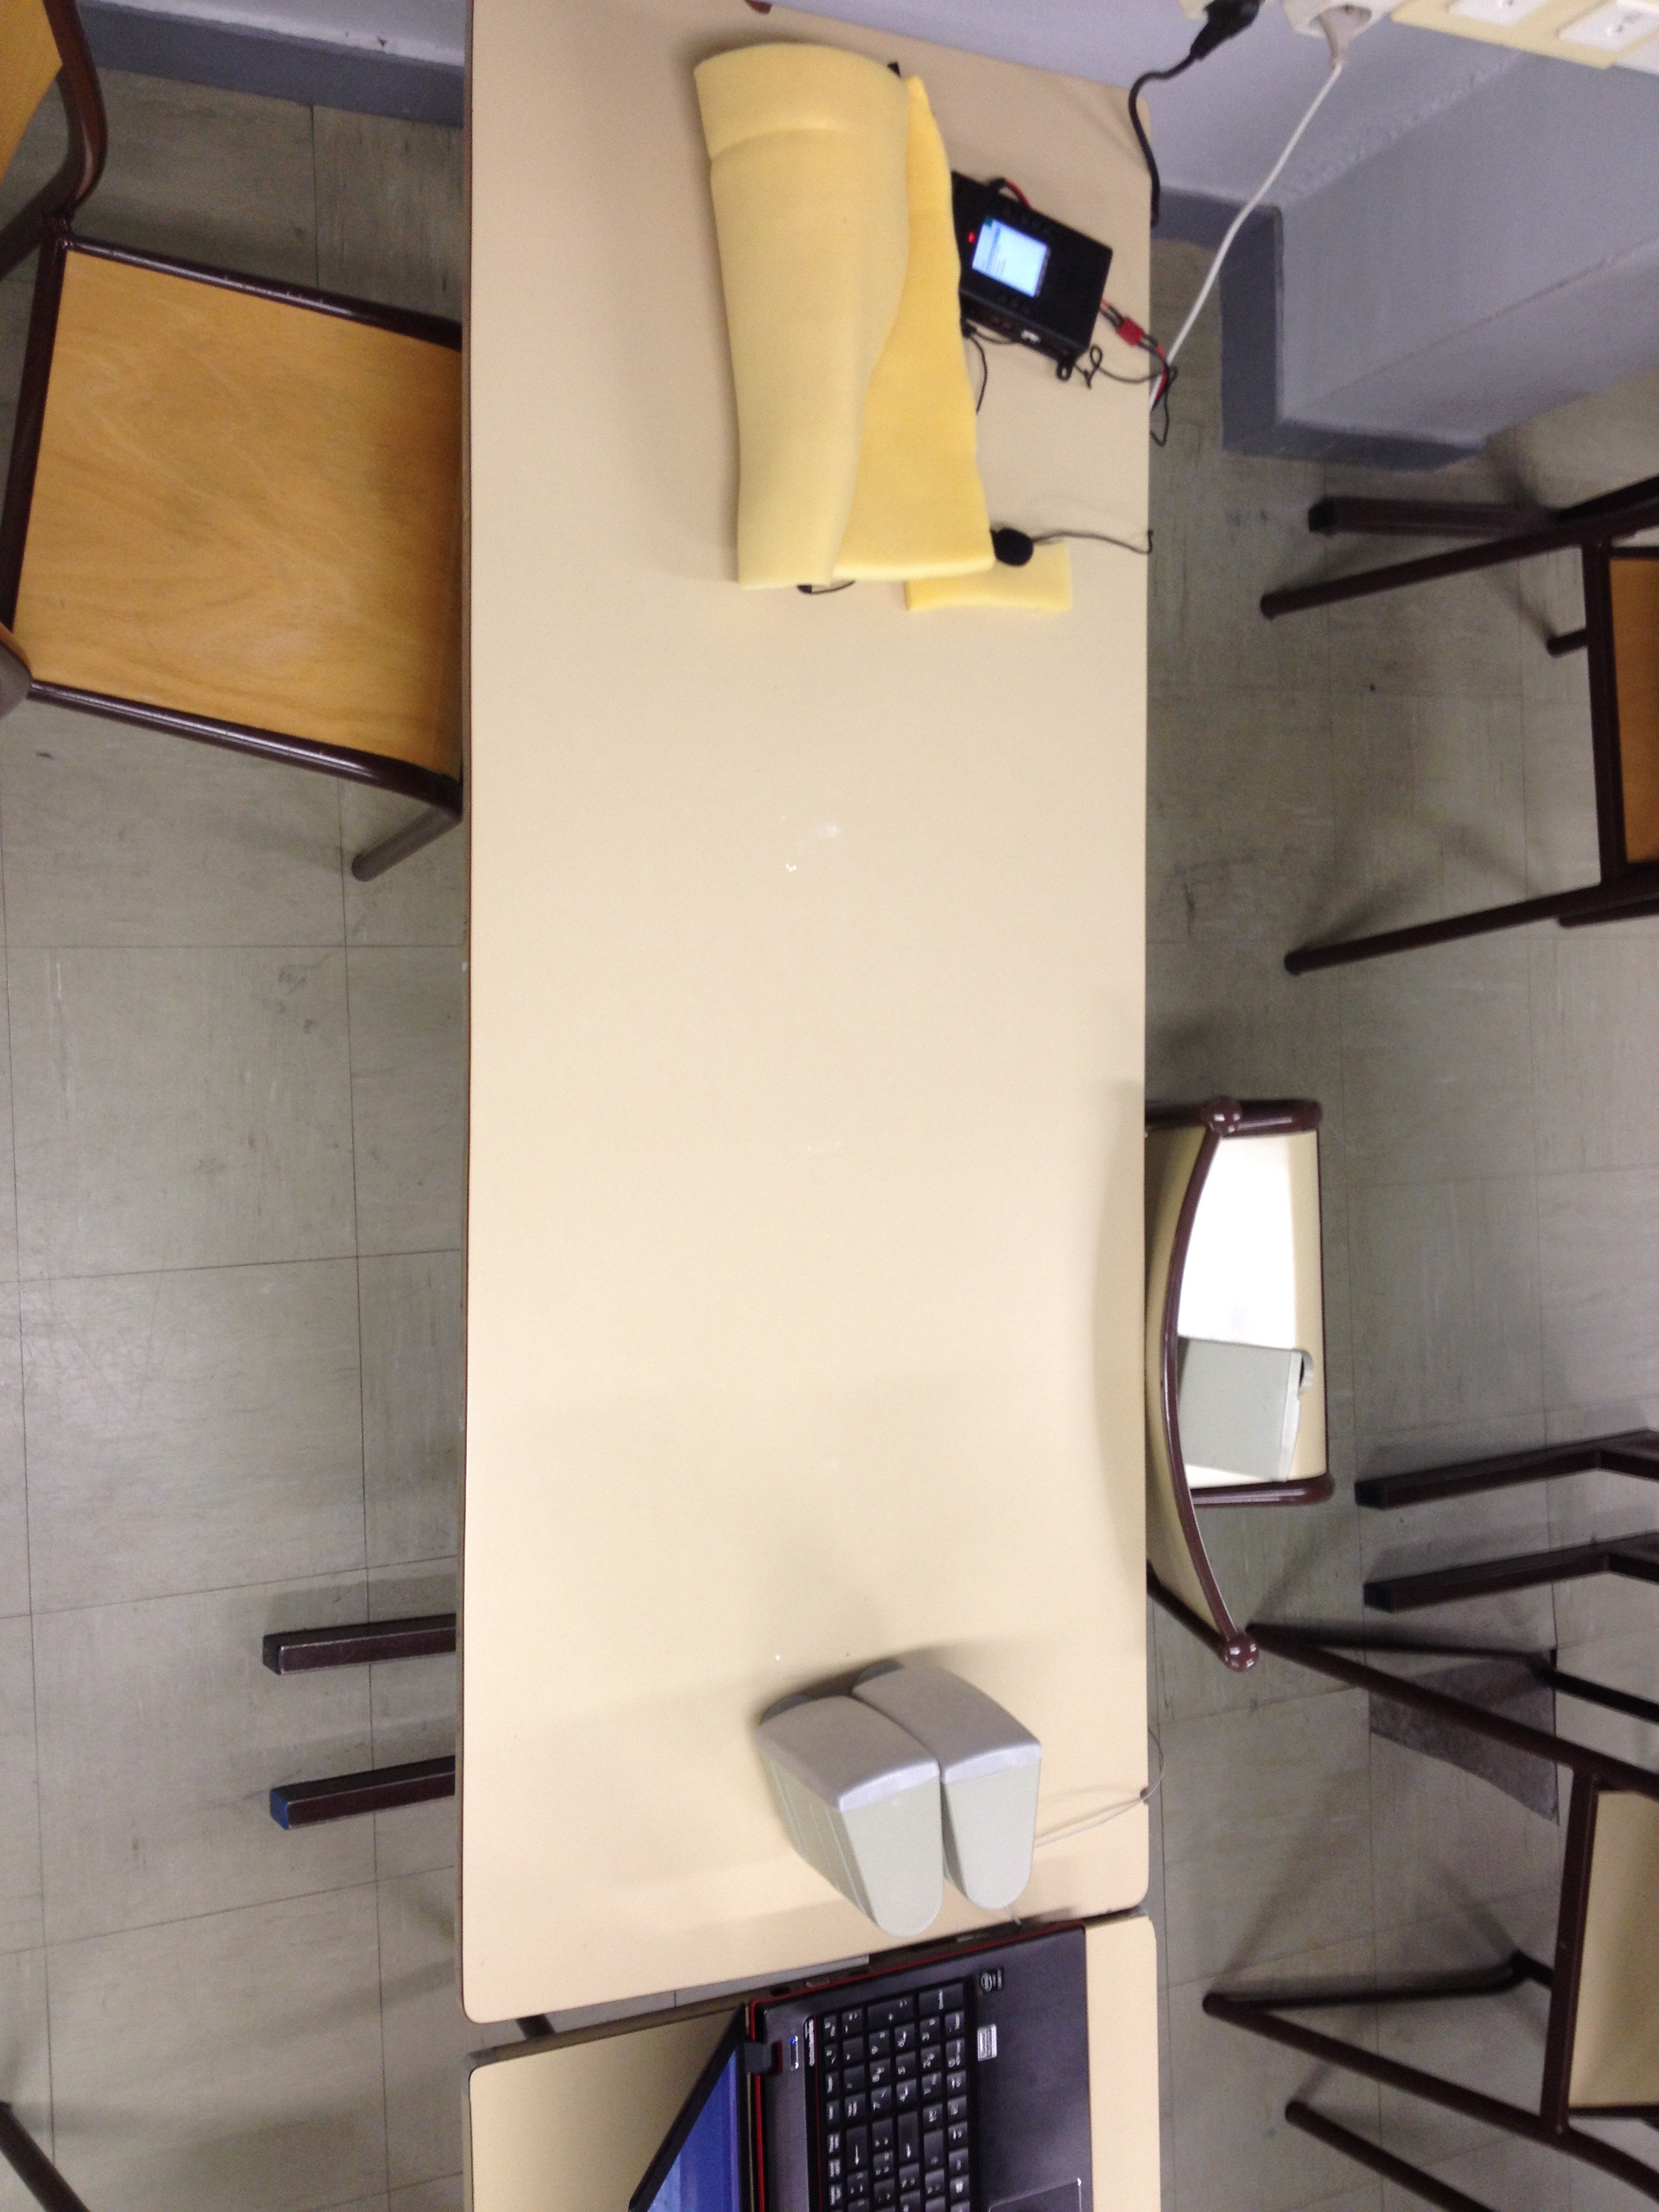
\includegraphics[width=\textwidth]{../donnees25-02/IMG_0924.jpg} 
\end{figure}

TODO: on a perdu certaines mesures, il va falloir les refaire :(

\subsection{conclusion}
On en conclu que l'écho influence effectivement beaucoup le signal reçu, pouvant fausser les calculs basés sur le décalage de phase.

\part{Signal carré}
\section{Objectifs}
	Le premier objectif de cette série de testes est de vérifier la validité de l'utilisation d'un signal carré.
	On a voulu tester cette forme de signal, car le front montant du signal est supposé être facilement repérable dans le signal de l'acquisition du micro.
	Le deuxième objectif est d'acquérir un signal avec le minimum d'écho possible. Le signal carré utilisé étant très court, le pique enregistré sur les micros ne devrait (hypothétiquement) pas être bruité par de l'écho.

\section{Protocole}
	On a créé deux fichier $.wav$:
	\begin{itemize}
	\item Le premier est composé d'une succession de signeaux carrée (de longueur 1 échantillon), chacune séparé de 3 secondes
	\item Le deuxieme est composé d'une succession de signeaux carrée (de longueur 5 echantillons) chacun séparé de 3 secondes
	\end{itemize}
	Tous les tests ont été effectué a distance de mures pour éviter la formation 
	On a ensuite fait les mêmes teste que pour les séances précédentes:

	
	
	

	premier test:
		les deux micros sont cote a cote(a 6cm de décalage), à la même distance de la source sonore.
\begin{figure}[H]
		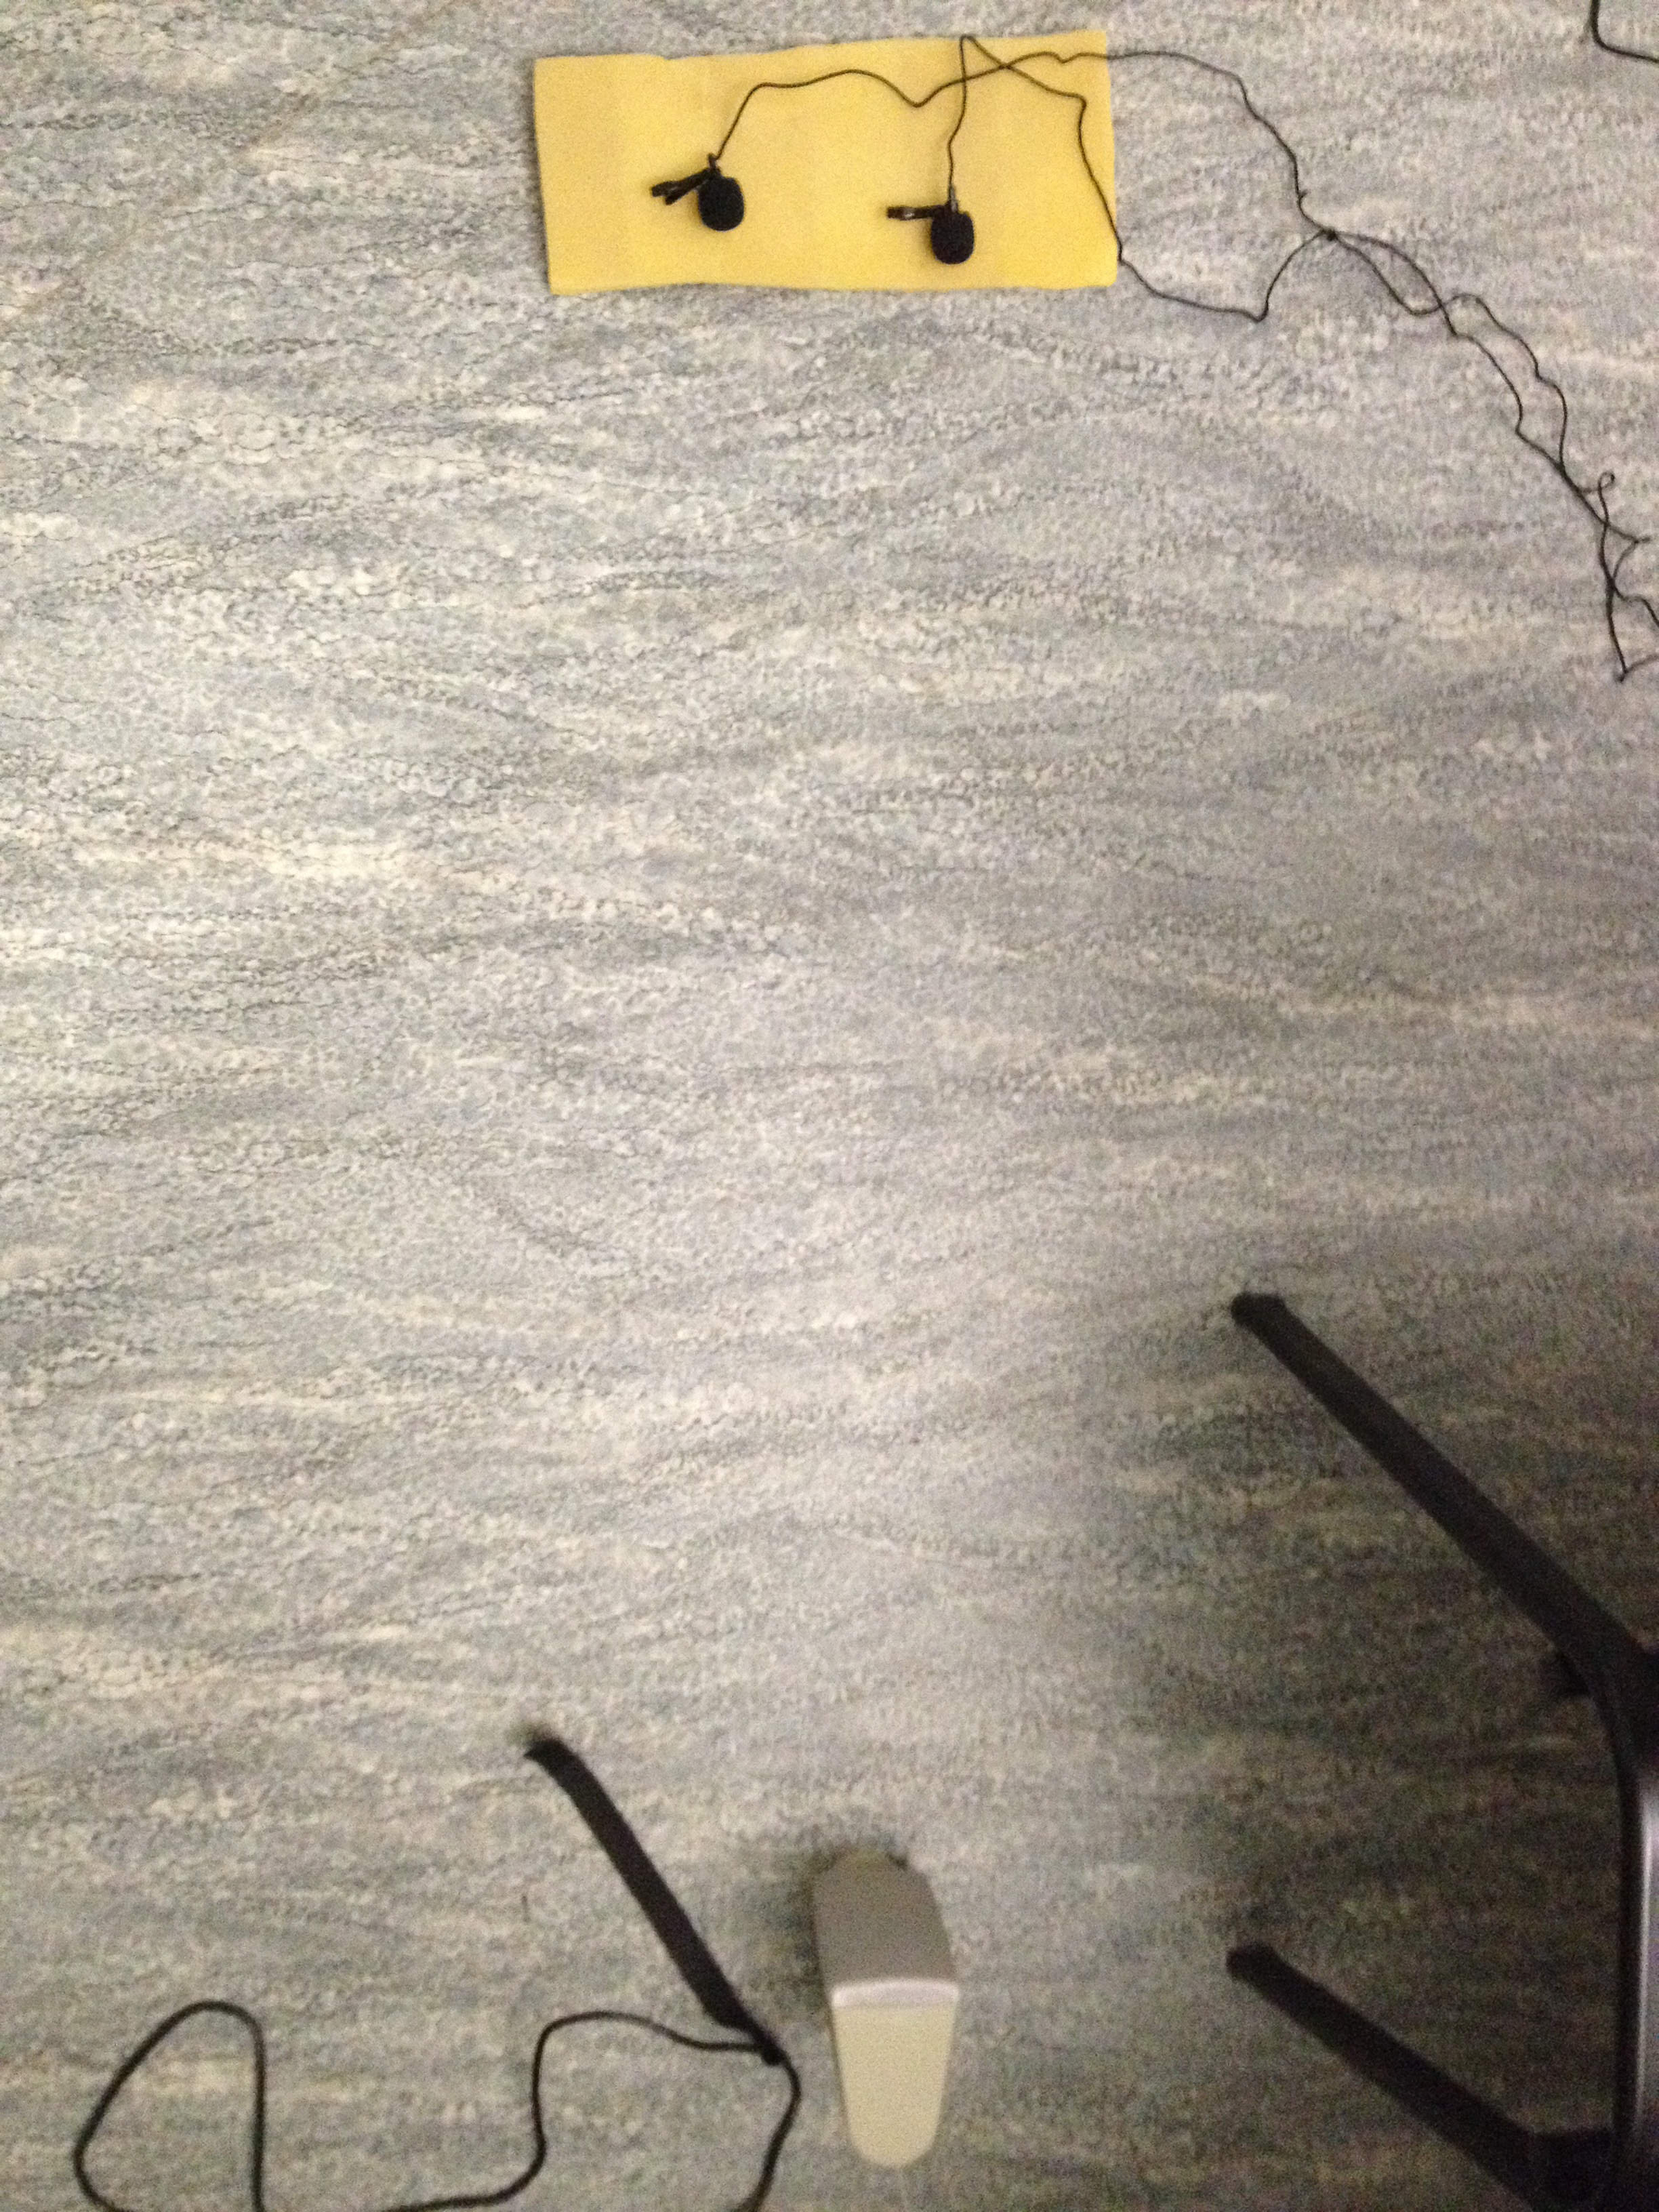
\includegraphics[width=\textwidth]{../donnees11-03/test_1.jpg} 
		\caption{photo de l'expérience avec les micros côte à côte}
\end{figure}
		
	deuxième test:
		les deux micros sont en ligne droite avec le speaker. la distance entre les deux micros est de 520mm, la distance entre le micro le plus proche du speaker et le speaker est de 400mm.
\begin{figure}[H]
		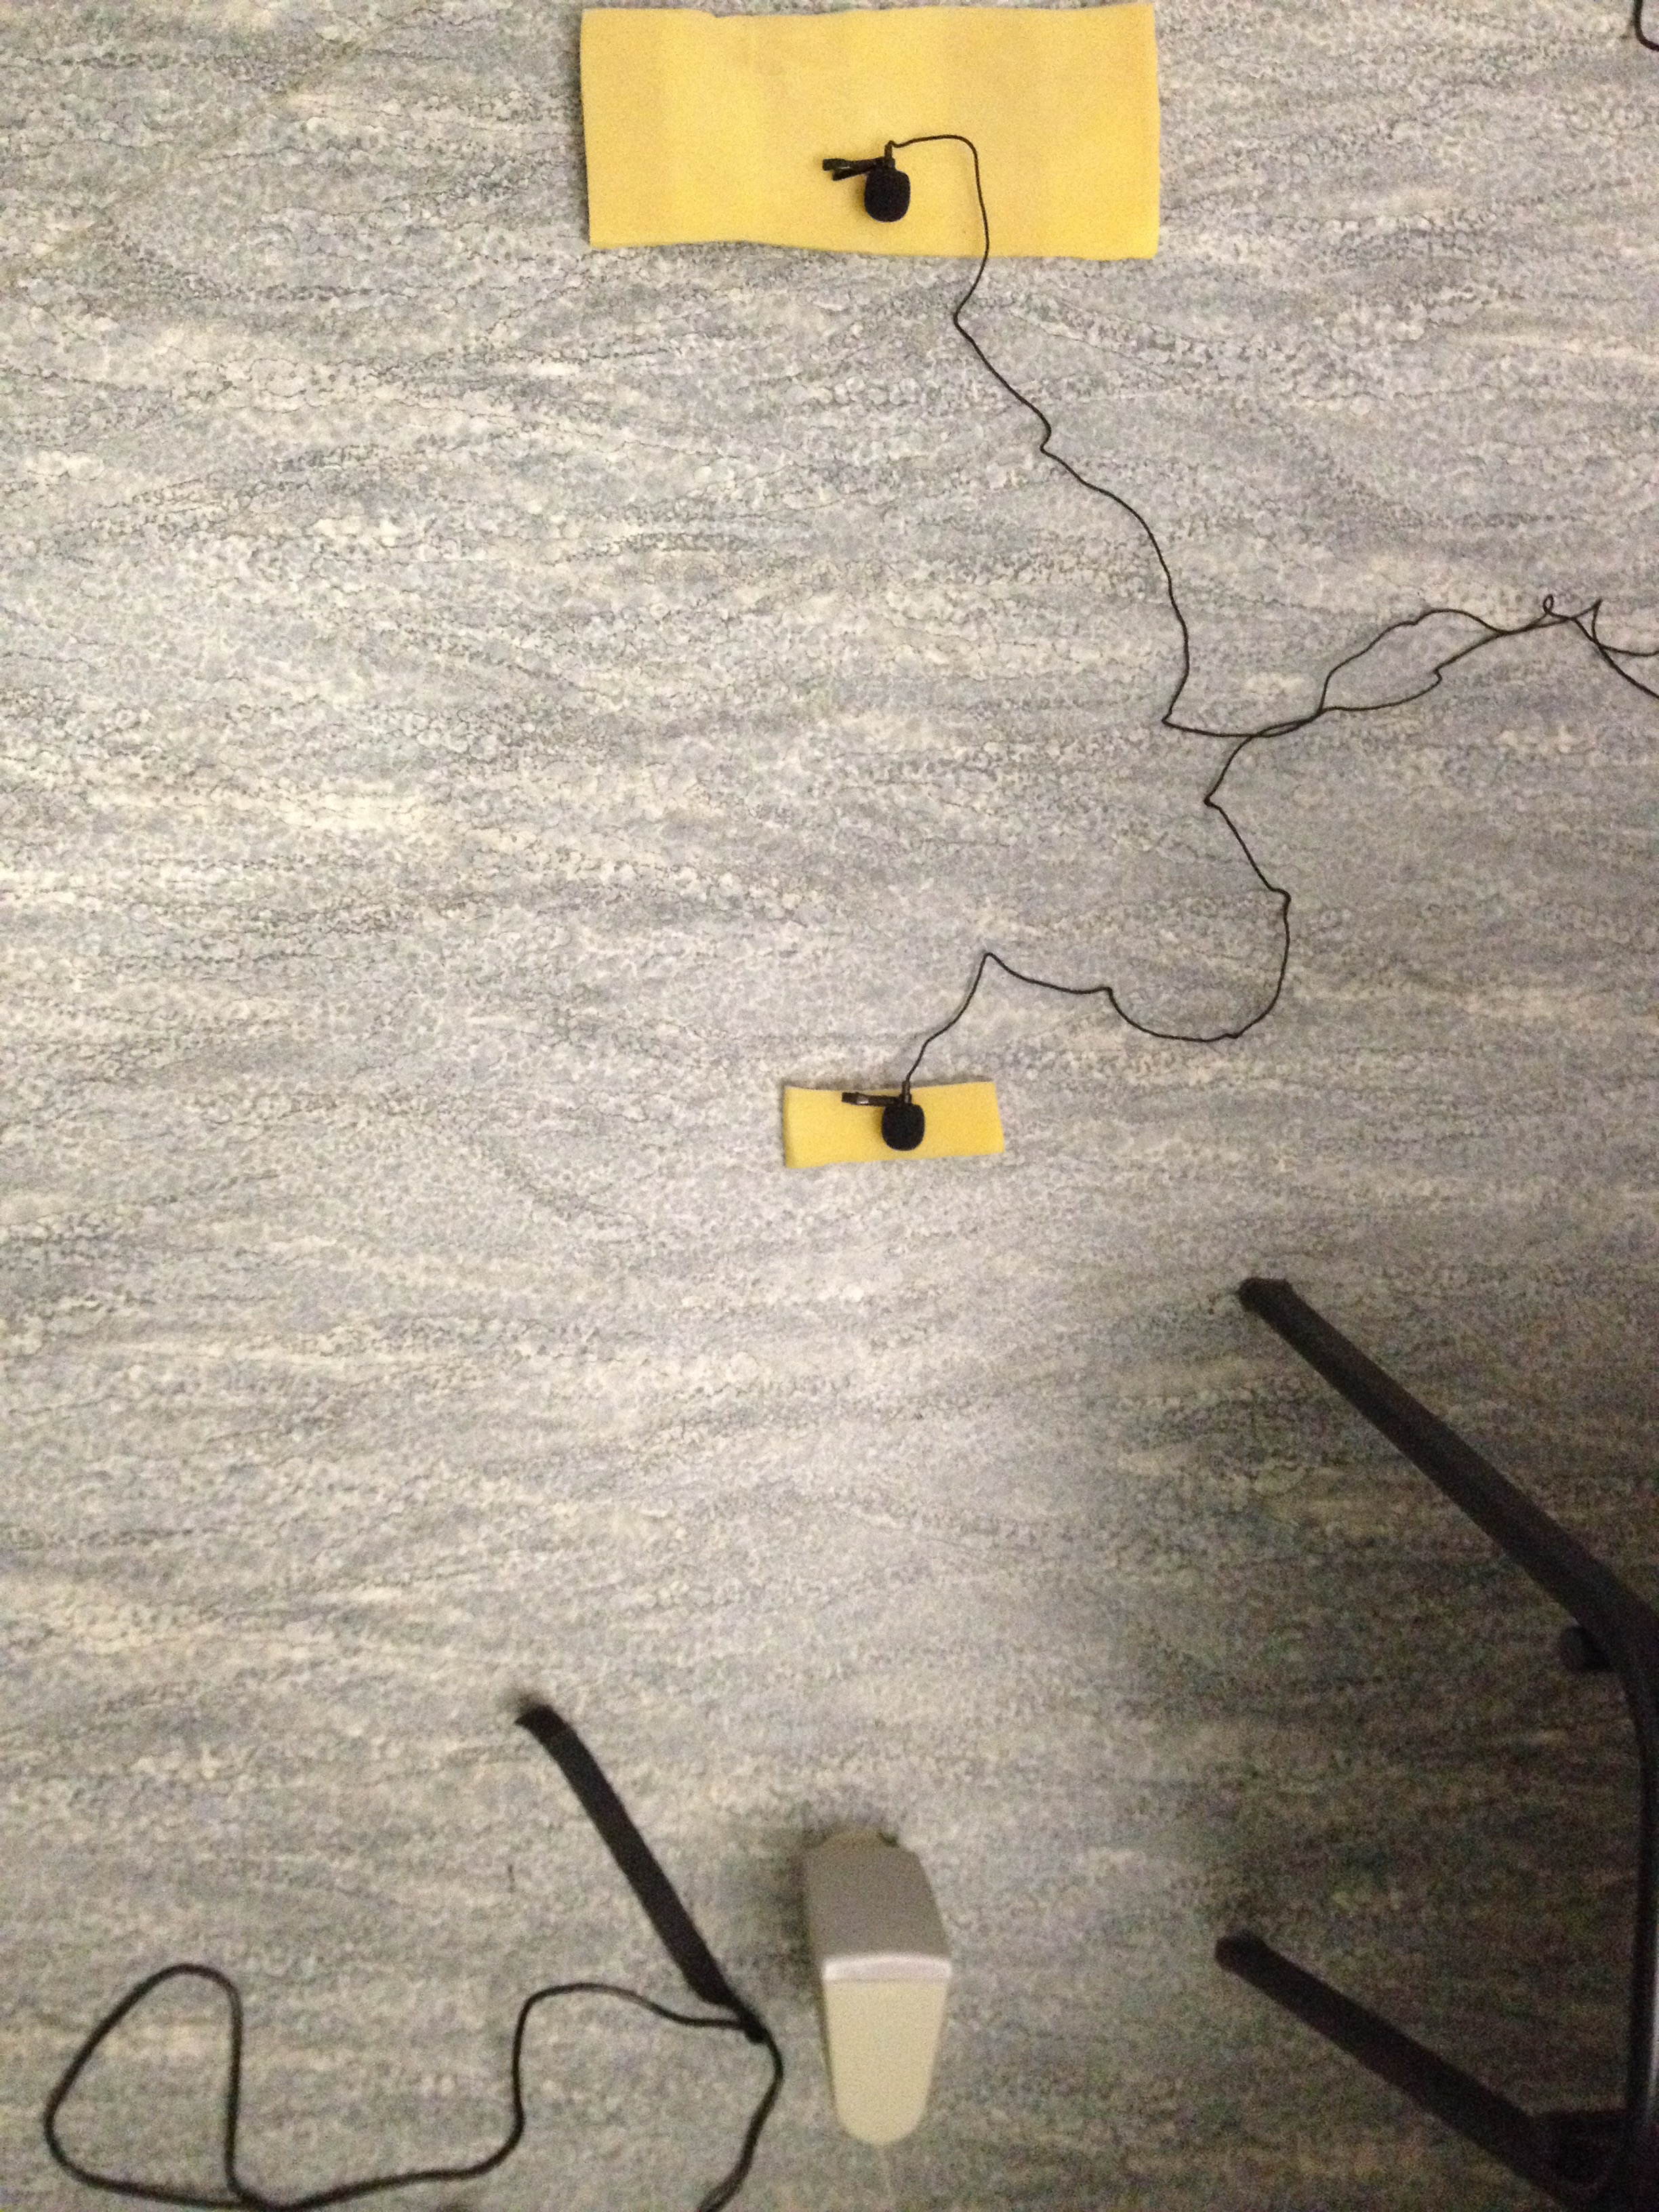
\includegraphics[width=\textwidth]{../donnees11-03/test_2.jpg} 
		\caption{photo de l'expérience avec les micros en ligne}
\end{figure}
	troisième test:
		les deux micros sont a la même distance par rapport a la source sonore(920mm), mais il sont tous les deux séparé de 680mm.

	quatrième test:
		un des deux micros est entouré de mousse pour faire un cône, le rendant unidirectionnel.
		le cône est dirigé vers le speaker
		les deux micros sont a une distance de 900mm.
\begin{figure}[H]
		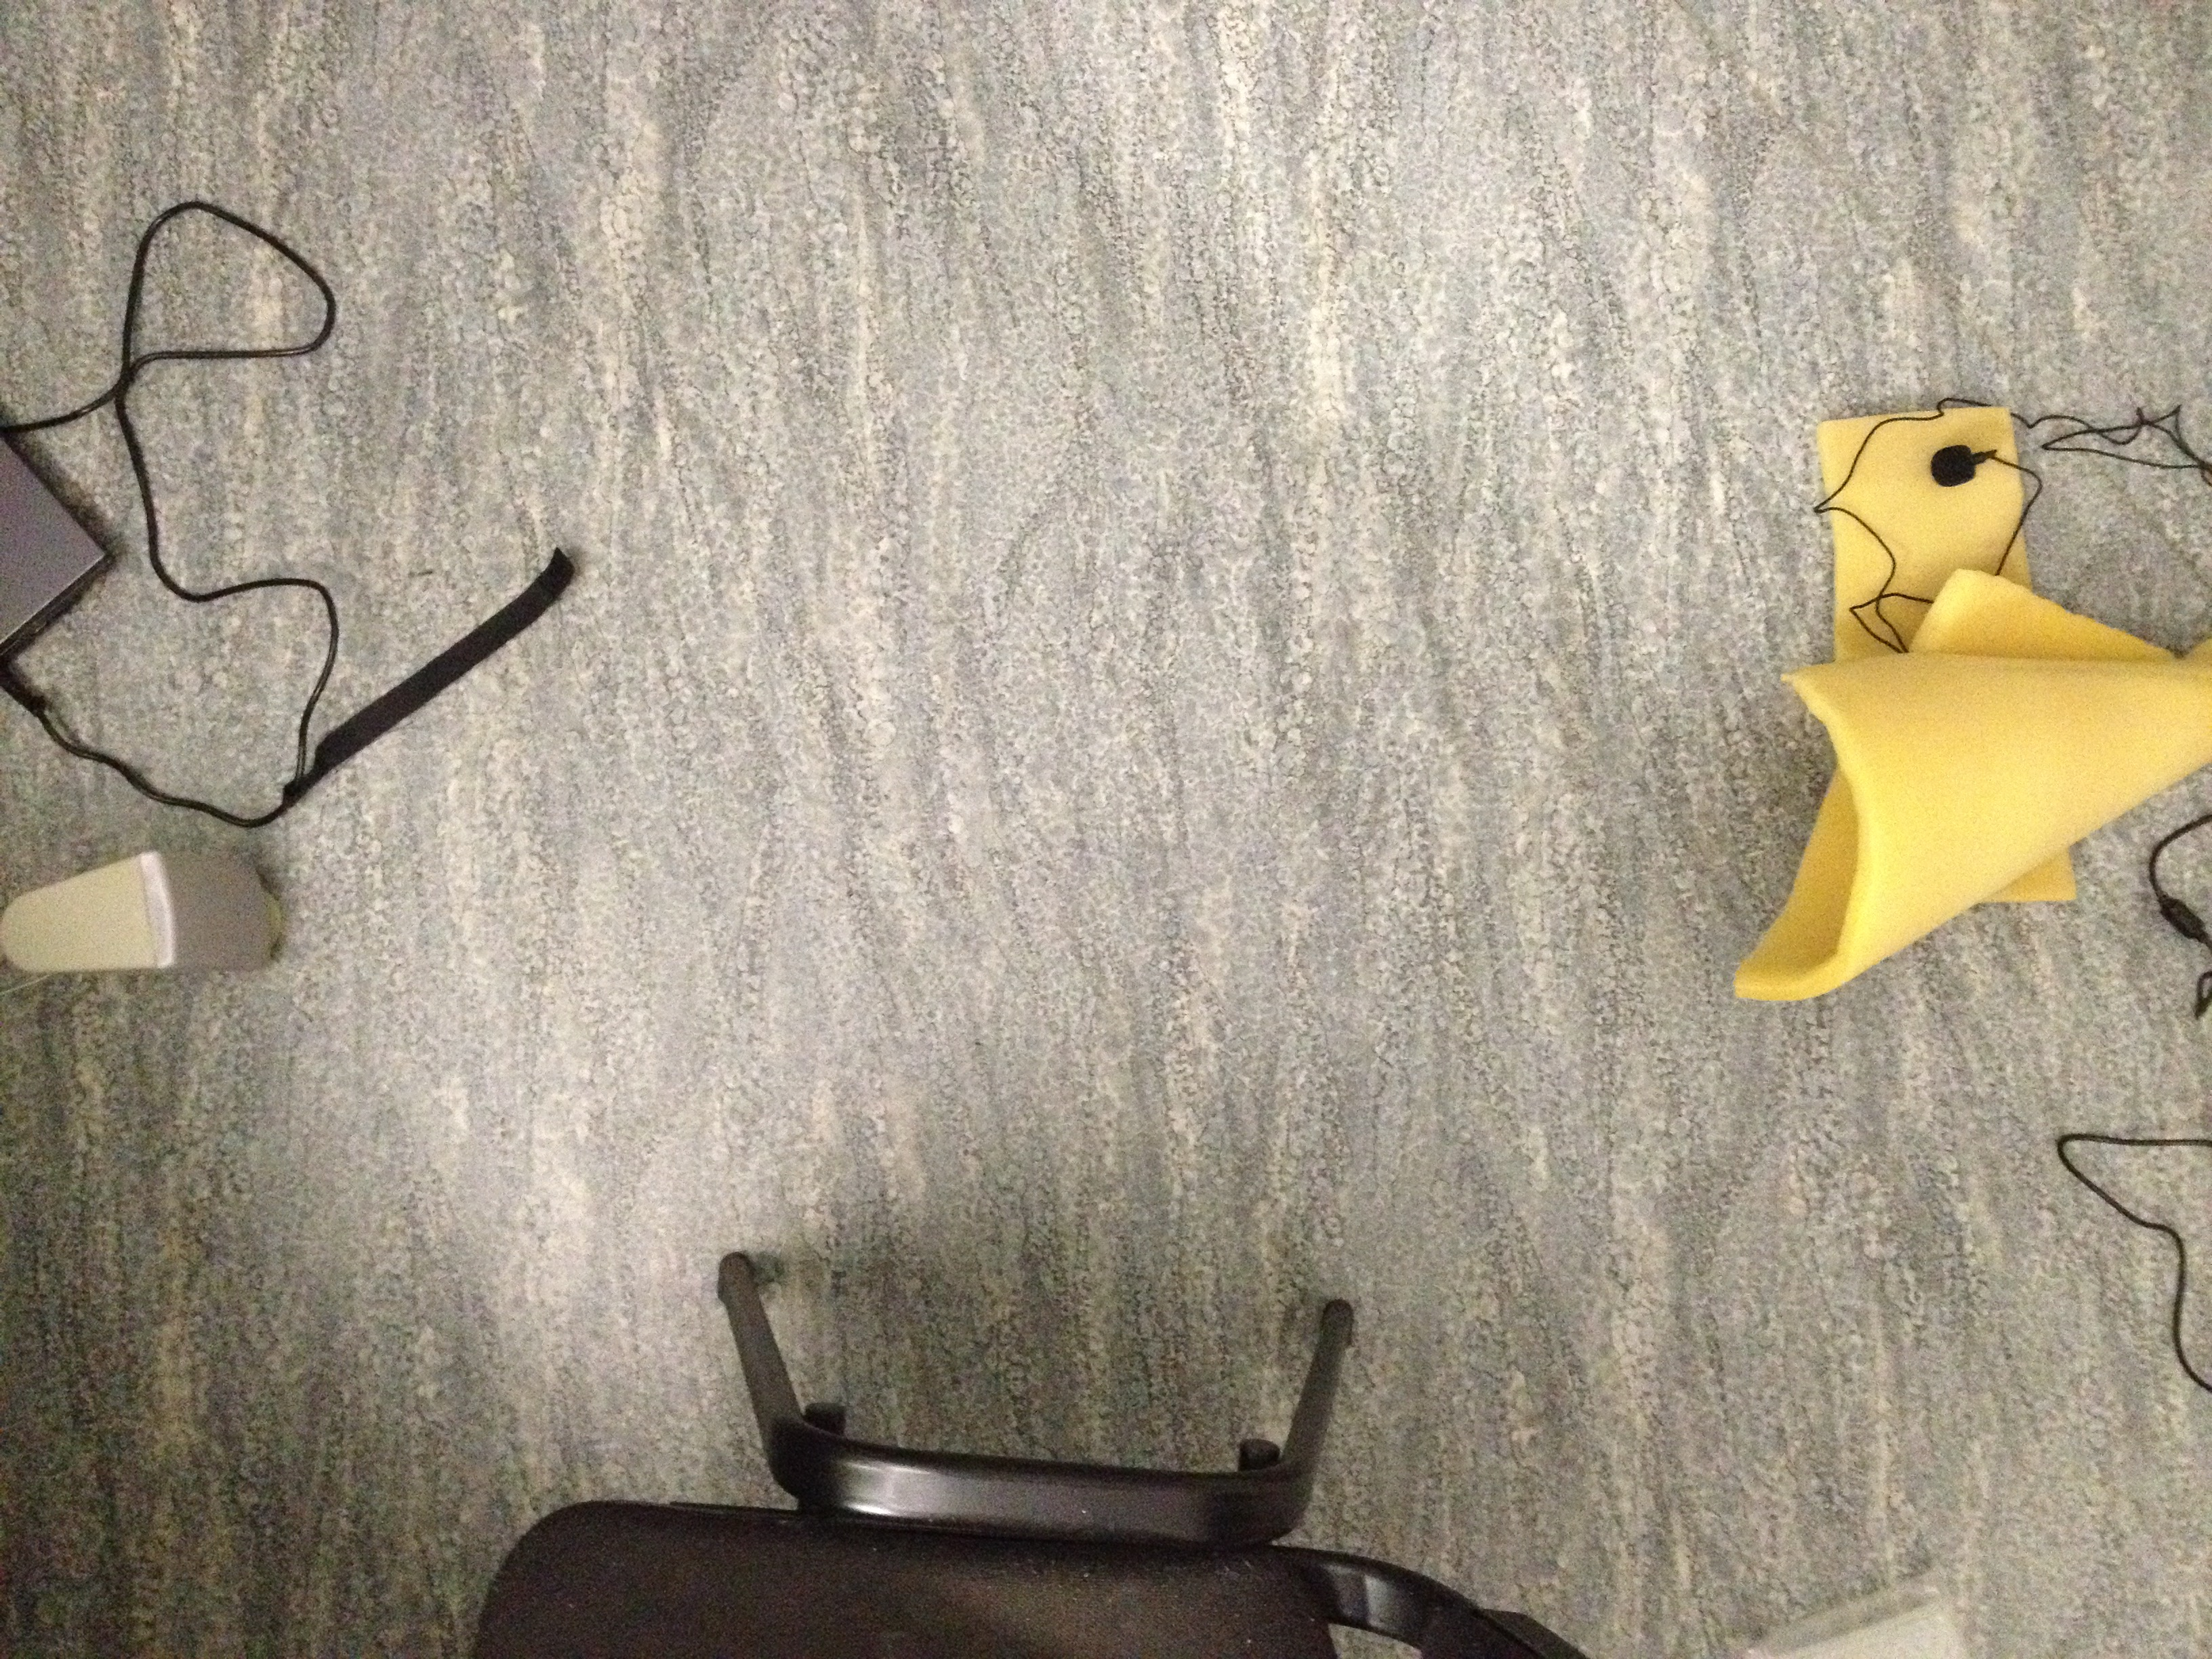
\includegraphics[width=\textwidth]{../donnees11-03/test_4.jpg} 
		\caption{photo de l'expérience avec un cône autour d'un micro}
\end{figure}
	cinquième test:
		un des deux micros est entouré de mousse pour faire un cone, le rendant unidirectionnel.
		le cone est dirigé a 180 degré du speaker.
		les deux micros sont a une distance de 900mm.


\section{Résultats/conclusions}
\paragraph{résultats}
	Impulsion carré de 1 sample:
		premier test:
			il n'y a un décalage que d'un sample entre les deux.

		deuxième test:
			le décalage de phase est de 11 sample, soit 220 microsecondes.

		troisième test:
			malgré le faite que les deux micros soient a la même distance avec la source sonore, il y a un décalage de phase de 2 sample. de plus, les deux signaux ne se ressemblent pas du tout!

		quatrième test :
			les deux signaux ne se ressemblent pas
			il y a décalage de 1 sample.

		cinquième test :
			le signal entouré du cone est beaucoup plus faible.
			il y a un décalage de 5 sample entre les deux signaux.

	Impulsion carré de 5 sample:
		premier test:
			il n'y a un décalage de phase que d'un seul sample. (20 microsecondes)

		deuxième test:
			le décalage de phase est de 11 sample (220 microsecondes)
			ce décalage de phase est cohérent avec la distance entre les deux micros

		troisième test:
			le décalage de phase est de 2 samples.
			de plus les deux signaux ne se ressemblent pas 

		quatrième test :
			il n' a pas de décalage de phase... je ne sais pas pourquoi!

		cinquième test :
	        le décalage de phase est de 2 sample. j'aurais pensé que ça soit plus.
	        le signale est beaucoup plus faible pour le micro qui est entouré du cone. 


\subsection{Conclusion}
	Malgré la forme du signal d'origine très reconnaissable, la signal reçu, l'est beaucoup moins. Il est assez compliqué de repéré le même extremum dans les deux signaux acquis par les micros.
	Le fait que le signal n'est pas reconnaissable, et que le tous les piques ne sont pas pareil dans l'enregistrement des deux micros, est probablement du au limitation matériel du haut parleur (la membrane vibre et ne peut pas reconstituer un signal carré)
	Malgré les effort pour limiter l'apparition d'écho, celui-ci est inévitable.



TODO: expliquer les pistes sur les captures d'écran audacity


\end{document}